\chapter{वायुदाब और मौसम}\label{ch:g5:air-pressure-weather}

तुम एक महासागर की तली में रहते हो --- \omterm{def:g2:air-around-us:air}{हवा} का महासागर, सैकड़ों
किलोमीटर गहरा, जिसका पूरा \omterm{def:g4:weight-and-mass:weight}{भार} तुम्हारे कंधों पर टिका है। वह तुम्हें
कुचल क्यों नहीं देता? तुम्हें उसका एहसास तक क्यों नहीं होता? और इस सब
का कल के मौसम से क्या लेना-देना है? \omterm{def:g2:air-around-us:air}{हवा}, हमारी वही पुरानी अनदेखी
दोस्त, एक और बड़ा राज़ खोलने वाली है।

\section{हवा का भार होता है}

\begin{example}[अनदेखे को तौलना]\label{ex:g5:air-pressure-weather:weighing}
कसा हुआ फ़ुटबॉल एक बारीक \omterm{def:g3:levers-and-scales:scale}{तुला} पर रखकर ठीक-ठीक \omterm{def:g2:balance-equilibrium:equilibrium}{संतुलित} किया जाता है।
फिर उसका वाल्व खोल दिया जाता है और भीतर की अतिरिक्त \omterm{def:g2:air-around-us:air}{हवा} सनसनाती हुई
निकल जाती है --- वही गेंद, वही वाल्व, सब कुछ वही, बस कुछ \omterm{def:g2:air-around-us:air}{हवा} कम। अब
फिर \omterm{def:g3:levers-and-scales:scale}{तुला} पर रखो: पिचकी हुई गेंद \emph{हल्की} है। यह फ़र्क़ भाग गई \omterm{def:g2:air-around-us:air}{हवा}
का \omterm{def:g4:weight-and-mass:weight}{भार} है। \omterm{def:g2:air-around-us:air}{हवा} पदार्थ है, पदार्थ का \omterm{def:g3:measuring-mass:mass}{द्रव्यमान} होता है, और \omterm{def:g3:measuring-mass:mass}{द्रव्यमान}
को पृथ्वी नीचे खींचती है: हमारे ऊपर वाला महासागर भारी है।
\end{example}

\begin{definition}[वायुमंडल और उसका दाब]\label{def:g5:air-pressure-weather:pressure}
\emph{वायुमंडल}\index{वायुमंडल} पूरी पृथ्वी के चारों ओर लिपटी \omterm{def:g2:air-around-us:air}{हवा} की
गहरी परत है। उसका \omterm{def:g4:weight-and-mass:weight}{भार} तली की \omterm{def:g2:air-around-us:air}{हवा} को --- यानी जहाँ हम रहते हैं, वहाँ की
\omterm{def:g2:air-around-us:air}{हवा} को --- दबा देता है, और दबी हुई \omterm{def:g2:air-around-us:air}{हवा} हर छूती हुई सतह पर ज़ोर से
धकेलती है। इसी धक्के को \emph{वायुदाब}\index{वायुदाब} कहते हैं।
\end{definition}

\begin{proposition}[हर ओर से धक्का]\label{prop:g5:air-pressure-weather:allsides}
\omterm{def:g5:air-pressure-weather:pressure}{वायुदाब} हर सतह पर \emph{हर} दिशा से धकेलता है --- मेज़ों पर नीचे की
ओर, दीवारों पर बग़ल से, और छतों तथा हथेलियों पर \emph{ऊपर} की ओर भी।
और वह ताक़तवर है: तुम्हारी हथेली जितने क्षेत्रफल पर \omterm{def:g2:air-around-us:air}{हवा} लगभग उतने ही
ज़ोर से धकेलती है जितना किसी बड़े, भरे हुए सूटकेस का \omterm{def:g4:weight-and-mass:weight}{भार} होता है। हमें
इसका पता इसलिए नहीं चलता कि धक्के बराबरी में आते हैं: हमारे भीतर की
और हर सतह के पीछे की \omterm{def:g2:air-around-us:air}{हवा} भी उतने ही ज़ोर से वापस धकेलती है।
\end{proposition}

\begin{method}[वह कार्ड जो पानी रोक लेता है]\label{met:g5:air-pressure-weather:card}
\omterm{def:g2:air-around-us:air}{हवा} का ऊपर की ओर धक्का, रँगे हाथों पकड़ा गया (इसे सिंक के ऊपर करो):
\begin{enumerate}
  \item एक गिलास को ऊपर किनारे तक पानी से भरो;
  \item उसके मुँह पर एक कड़ा, चिकना कार्ड सपाट रखो, जो चारों ओर पानी
        को छूता हो;
  \item कार्ड को अपनी जगह थामे रखो, गिलास को ठीक उलटा करो, और फिर
        धीरे से कार्ड छोड़ दो।
\end{enumerate}
कार्ड टिका रहता है --- और पूरा गिलास भर पानी रोके रखता है। पानी का \omterm{def:g4:weight-and-mass:weight}{भार}
कार्ड को नीचे दबाता है, पर \omterm{def:g5:air-pressure-weather:pressure}{वायुमंडल} उसे \emph{ऊपर} की ओर उससे भी
ज़्यादा ज़ोर से दबाता है। तुमने अभी सूटकेस वाला वही धक्का नीचे से देख
लिया।
\end{method}

\begin{omfigure}
\begin{tikzpicture}[scale=0.85]
  \draw[thick] (4.4,1.2) -- (4.4,3.6) (6.6,1.2) -- (6.6,3.6);
  \draw[thick] (4.4,3.6) -- (6.6,3.6);
  \fill[omDef, opacity=0.25] (4.4,1.25) rectangle (6.6,3.55);
  \draw[very thick, omMeth] (4.25,1.2) -- (6.75,1.2);
  \node[right, font=\small, omMeth] at (6.9,1.2) {कार्ड};
  \draw[-Stealth, thick, omDef] (5.0,2.9) -- (5.0,2.2);
  \draw[-Stealth, thick, omDef] (6.0,2.9) -- (6.0,2.2);
  \node[above, font=\small, omDef] at (5.5,3.65)
    {पानी नीचे धकेलता है};
  \foreach \x in {4.7,5.5,6.3} {
    \draw[-Stealth, very thick, omThm] (\x,0.15) -- (\x,0.95);
  }
  \node[below, font=\small, omThm] at (5.5,-0.05)
    {वायुमंडल ऊपर धकेलता है --- ज़्यादा ज़ोर से};
\end{tikzpicture}

{\small उलटा किया गया गिलास: कार्ड पर \omterm{def:g2:air-around-us:air}{हवा} का ऊपर की ओर धक्का पानी के
\omterm{def:g4:weight-and-mass:weight}{भार} को मात दे देता है। अनदेखा महासागर ताक़तवर है।}
\end{omfigure}

\section{वायुमंडल से चलने वाले यंत्र}

\begin{example}[नली]\label{ex:g5:air-pressure-weather:straw}
तुम्हें लगता है कि तुम नली से रस ऊपर खींचते हो। सच यह है कि \omterm{def:g3:solids-liquids-gases:liquid}{द्रव} को
खींचा जा ही नहीं सकता --- उँगलियों से पानी खींचकर देख लो! तुम असल में
नली में से \emph{\omterm{def:g2:air-around-us:air}{हवा}} चूस लेते हो। भीतर से \omterm{def:g2:air-around-us:air}{हवा} जाते ही, गिलास के रस
पर नीचे की ओर दबाता \omterm{def:g5:air-pressure-weather:pressure}{वायुमंडल} उस ख़ाली नली में रस को ऊपर तुम्हारे मुँह
तक धकेल देता है। हर घूँट में उठाने का काम \omterm{def:g5:air-pressure-weather:pressure}{वायुमंडल} करता है; तुम तो बस
रास्ता ख़ाली करते हो।
\end{example}

\begin{example}[चूषण-कप और पिचकी बोतलें]\label{ex:g5:air-pressure-weather:suction}
स्नानघर के हुक का रबर वाला कप टाइलों से सटाकर दबाया जाता है, जिससे
उसके नीचे की \omterm{def:g2:air-around-us:air}{हवा} निकल जाती है: अब \omterm{def:g5:air-pressure-weather:pressure}{वायुमंडल} उस कप को दीवार से चिपकाए
रखता है और पीछे से वापस धकेलने वाला कोई नहीं बचता --- यानी उसे आकाश ने
ही ठोंक रखा है। और पहाड़ पर ऊँचाई पर किसी ख़ाली प्लास्टिक बोतल का
ढक्कन कसकर बंद करो, फिर घाटी में उतर आओ: बोतल ऐसे पिचक जाती है मानो
किसी अनदेखे हाथ ने दबा दी हो। बाहर की \omterm{def:g2:air-around-us:air}{हवा} भीतर बंद पतली पहाड़ी \omterm{def:g2:air-around-us:air}{हवा} से
ज़्यादा ज़ोर से दबाती है --- \omterm{def:g5:air-pressure-weather:pressure}{वायुमंडल} जीत जाता है, और बोतल मुड़ जाती
है।
\end{example}

\begin{example}[ऊँचाई के साथ पतली होती हवा]\label{ex:g5:air-pressure-weather:height}
ऊपर चढ़ो, और महासागर का कुछ हिस्सा तुम्हारे नीचे रह जाता है: ऊपर कम
\omterm{def:g2:air-around-us:air}{हवा} यानी कमज़ोर धक्का। तेज़ चलती रोपवे की गाड़ी में बाहरी दाब बदलते
ही तुम्हारे कान चटक जाते हैं; और पर्वतारोही पतली पड़ चुकी \omterm{def:g2:air-around-us:air}{हवा} में
हाँफते हैं। यहीं पिछले साल वाली पहाड़ी चाय की पहेली हथियार डाल देती
है: \omterm{def:g5:air-pressure-weather:pressure}{वायुमंडल} पानी पर कम दबाता है, इसलिए उबलना आसान हो जाता है ---
ऊँची चोटियों पर पानी \qty{100}{\celsius} से काफ़ी नीचे ही उबल जाता
है, यानी ढंग की चाय बनाने के लिए बहुत ठंडा।
\end{example}

\begin{omfigure}
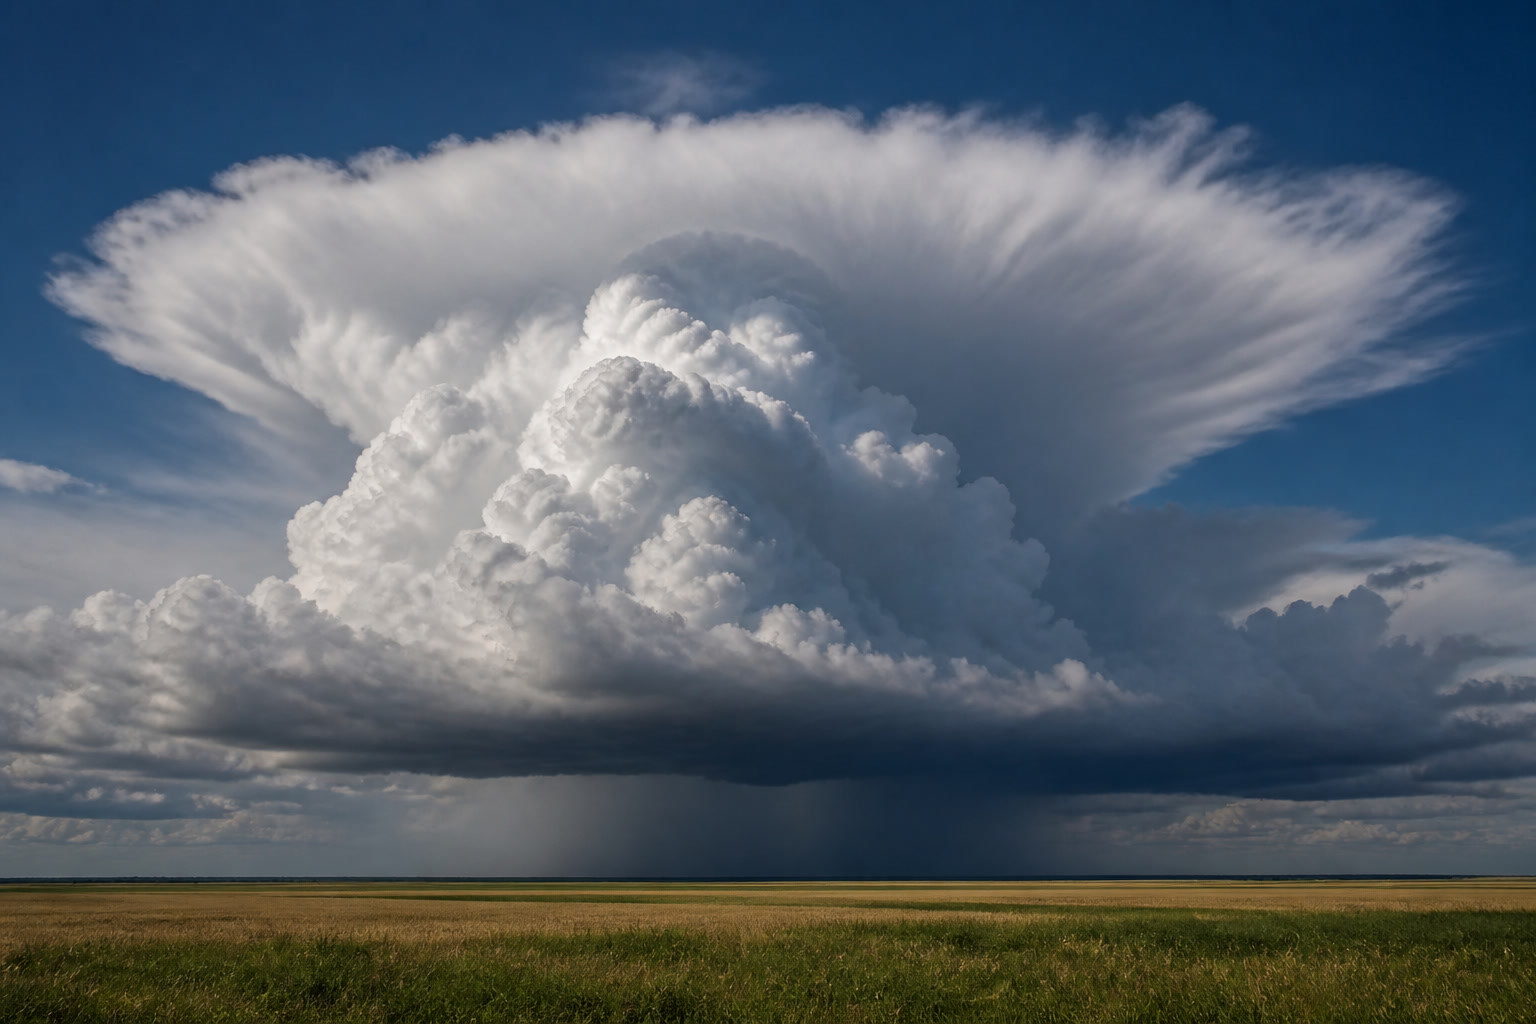
\includegraphics[width=0.58\linewidth]{images/book1/ai/g5-weather-storm.jpg}

{\small खेतों के ऊपर तनी हुई गरजती बदली: मौसम असल में चलता-फिरता \omterm{def:g5:air-pressure-weather:pressure}{वायुमंडल} ही है।}
\end{omfigure}

\section{दाबमापी और मौसम}

\begin{definition}[दाबमापी]\label{def:g5:air-pressure-weather:barometer}
\emph{दाबमापी}\index{दाबमापी} वह उपकरण है जो \omterm{def:g5:air-pressure-weather:pressure}{वायुदाब} मापता है ---
\omterm{def:g3:temperature-thermometers:temperature}{तापमापी} और \omterm{def:g3:levers-and-scales:scale}{तुला} के बग़ल में खड़ा हमारे ईमानदार जजों के कुनबे का एक और
सदस्य। ऊपर का \omterm{def:g5:air-pressure-weather:pressure}{वायुमंडल} ज़्यादा ज़ोर से दबाए तो उसकी सुई चढ़ती है, और
दबाव हल्का पड़े तो गिरती है।
\end{definition}

\begin{proposition}[दाब कल की बात करता है]\label{prop:g5:air-pressure-weather:weather}
\omterm{def:g5:air-pressure-weather:pressure}{वायुमंडल} का दाब बेचैन रहता है: भारी, नीचे बैठती \omterm{def:g2:air-around-us:air}{हवा} शांत और साफ़
आकाश लाती है; हल्की, ऊपर उठती \omterm{def:g2:air-around-us:air}{हवा} बादलों और बारिश को न्योता देती है।
इसलिए \omterm{def:g5:air-pressure-weather:barometer}{दाबमापी} एक \omterm{def:g3:solids-liquids-gases:solid}{ठोस} और ईमानदार क़िस्म का भविष्यवक्ता है: \emph{ठहरा
हुआ या चढ़ता} दाब अच्छे मौसम का वादा करता है; \emph{गिरता} दाब बादलों
के आने की चेतावनी देता है; और \emph{तेज़ी से गिरता} दाब बताता है कि
तूफ़ान रास्ते में हो सकता है।
\end{proposition}

\begin{omfigure}
\begin{tikzpicture}[scale=0.85]
  \draw[thick] (2.2,1.7) circle (1.5);
  \foreach \a/\t in {150/{}, 120/{}, 90/{}, 60/{}, 30/{}} {
    \draw (2.2,1.7) ++(\a:1.3) -- ++(\a:0.18);
  }
  \node[font=\footnotesize] at (1.1,2.6) {बारिश};
  \node[font=\footnotesize] at (2.2,3.0) {बदलाव};
  \node[font=\footnotesize] at (3.4,2.6) {साफ़};
  \draw[-Stealth, very thick, omThm] (2.2,1.7) -- ++(55:1.1);
  \fill (2.2,1.7) circle (2pt);
  \node[below, font=\small] at (2.2,-0.05)
    {घर का दाबमापी: सुई साफ़ मौसम की ओर झुकी है};
  \node[right, font=\small, align=left] at (5.4,2.5)
    {चढ़ती सुई: आगे साफ़ आकाश};
  \node[right, font=\small, align=left] at (5.4,1.7)
    {गिरती सुई: बादल जुट रहे हैं};
  \node[right, font=\small, align=left] at (5.4,0.9)
    {तेज़ी से गिरती सुई: सँभल जाओ --- तूफ़ान};
\end{tikzpicture}

{\small \omterm{def:g5:air-pressure-weather:barometer}{दाबमापी} पढ़ना: असली बात यह नहीं कि सुई कहाँ खड़ी है, बल्कि यह
कि वह किस ओर सरक रही है --- \omterm{def:g5:air-pressure-weather:pressure}{वायुमंडल} अपनी योजनाएँ बता देता है।}
\end{omfigure}

\begin{remark}[मौसम के नक़्शे वाले H और L]\label{rem:g5:air-pressure-weather:map}
आज रात का मौसम बुलेटिन बड़े-बड़े घुमाव दिखाएगा, जिन पर H और L लिखा
होगा: ऊँचे और नीचे दाब वाले इलाक़े, जो नक़्शे पर सुस्त व्हेलों की तरह
सरकते रहते हैं। \omterm{def:g2:air-around-us:air}{हवा} हमेशा भारी H इलाक़ों से हल्के L इलाक़ों की ओर
उँडेलती रहती है --- और वही उँडेलना \emph{\omterm{def:g2:air-around-us:wind}{पवन} है}। एक ही अध्याय, और तीन
पुराने दोस्तों की व्याख्या: \omterm{def:g5:air-pressure-weather:barometer}{दाबमापी} की भविष्यवाणी, \omterm{def:g2:air-around-us:wind}{पवन} का जन्म, और वह
वजह जिससे तुम्हारे कान पहले ही जान जाते हैं कि मौसम बिगड़ने वाला है।
\end{remark}

\section{अभ्यास}

\begin{exercise}[$\star$]\label{exo:g5:air-pressure-weather:1}
फ़ुटबॉल वाला प्रयोग कैसे दिखाता है कि \omterm{def:g2:air-around-us:air}{हवा} का \omterm{def:g4:weight-and-mass:weight}{भार} होता है? ठीक-ठीक
किसकी तुलना की जाती है?
\end{exercise}

\begin{exercise}[$\star$]\label{exo:g5:air-pressure-weather:2}
\omterm{def:g5:air-pressure-weather:pressure}{वायुदाब} क्या है, और वह आता कहाँ से है? वह किन दिशाओं में धकेलता है?
\end{exercise}

\begin{exercise}[$\star$]\label{exo:g5:air-pressure-weather:3}
\omterm{def:g5:air-pressure-weather:pressure}{वायुमंडल} तुम्हारी हथेली पर लगभग उतने ही ज़ोर से दबाता है जितना किसी
भरे सूटकेस का \omterm{def:g4:weight-and-mass:weight}{भार} होता है --- फिर भी तुम्हें कुछ महसूस नहीं होता।
क्यों नहीं?
\end{exercise}

\begin{exercise}[$\star$]\label{exo:g5:air-pressure-weather:4}
कार्ड वाली तरकीब में दो धक्के कार्ड के लिए लड़ते हैं। उनके नाम बताओ,
और कहो कि जीतता कौन है।
\end{exercise}

\begin{exercise}[$\star$]\label{exo:g5:air-pressure-weather:5}
``मैं नली से रस ऊपर खींचता हूँ।'' इस वाक्य को सुधारो: तुम असल में
क्या हटाते हो, और उठाने का काम कौन करता है?
\end{exercise}

\begin{exercise}[$\star$]\label{exo:g5:air-pressure-weather:6}
चूषण-कप टाइलों को क्यों पकड़ लेता है? बाहर क्या निकाला गया, और कप को
थामे कौन रखता है?
\end{exercise}

\begin{exercise}[$\star$]\label{exo:g5:air-pressure-weather:7}
पहाड़ पर चढ़ते समय \omterm{def:g5:air-pressure-weather:pressure}{वायुदाब} का क्या होता है, और क्यों? यात्री को दिखने
वाले उसके दो सुराग़ बताओ।
\end{exercise}

\begin{exercise}[$\star$]\label{exo:g5:air-pressure-weather:8}
\omterm{def:g5:air-pressure-weather:barometer}{दाबमापी} क्या मापता है? नाश्ते से लेकर अब तक तुम्हारा \omterm{def:g5:air-pressure-weather:barometer}{दाबमापी} तेज़ी से
गिर रहा है --- सैर-सपाटे की योजनाओं को क्या उम्मीद रखनी चाहिए?
\end{exercise}

\begin{exercise}[$\star\star$]\label{exo:g5:air-pressure-weather:9}
पहाड़ से नीचे उतरते समय बंद बोतल पिचक गई। भीतर और बाहर के धक्कों से
इस पिचकने की व्याख्या करो --- और यह भी बताओ कि घाटी में बंद की गई और
\emph{ऊपर} ले जाई गई बोतल के साथ इसके उलट क्या होगा।
\end{exercise}

\begin{exercise}[$\star\star$]\label{exo:g5:air-pressure-weather:10}
मौसम के नक़्शे के H और L घुमावों के अनुसार \omterm{def:g2:air-around-us:wind}{पवन} आती कहाँ से है? इसे इस
पुस्तक की सबसे पुरानी परिभाषा से जोड़ो: \omterm{def:g2:air-around-us:wind}{पवन} यानी चलती हुई \omterm{def:g2:air-around-us:air}{हवा} ---
पर उसे चलाता कौन है?
\end{exercise}

\begin{exercise}[$\star\star$]\label{exo:g5:air-pressure-weather:11}
पर्वतारोही शिकायत करते हैं कि ऊँची चोटियों पर चाय कभी कड़क नहीं बनती
और सिवइयाँ कितनी भी देर उबालो कच्ची ही रहती हैं। दो वर्षों में फैली
पूरी व्याख्या इकट्ठी करो: पतला \omterm{def:g5:air-pressure-weather:pressure}{वायुमंडल} \omterm{def:g4:changes-of-state:boiling-point}{क्वथनांक} के साथ क्या करता है,
और ज़्यादा देर उबालने से मदद क्यों नहीं मिलती? (दो प्रतिज्ञप्तियाँ,
जिनमें से एक पिछले साल की है, यह मुक़दमा बंद कर देती हैं।)
\end{exercise}
